\chapter{Hardware Model and Implementation}

This chapter details the hardware designed during this Master's thesis to accelerate neural network training. The current hardware implements both training and inference acceleration for the neural network architecture described in section \ref{net-arch}.
\todo[inline]{Refer to github, appendix, and project link}
\section{Specifications}
The hardware model was implemented using a ZedBoard. The ZedBoard is a development board equipped with a Zynq-7000 XC7Z020 SoC. The Zynq series has both a processing system and programmable logic, where the processing system is a ARM Cortex-A9 based processor (hereafter referred to as the ``PS'') and the programmable logic is an Artix-7 series FPGA. Bitstreams for the FPGA were generated using Vivado 2018.3 and PetaLinux boot images for the PS were created using Xilinx SDK. The hardware description language (HDL) code for the project was primarily written in SystemVerilog. The programs run on the PS were written in C.
\todo[inline]{Cite the datasheets}

\section{The Implemented Neural Network}\label{net-arch}
\todo[inline]{MACs of the networks, distribution of kernels, probably to go in analysis}
\todo[inline]{figure of network.}

\section{Design Goals}
There were a few key principles that guided the overall design process throughout the development of the hardware accelerator. A core tenet was to maintain the project such that in the future HDL could be generated for training a network of any architecture so long as the desired layer types had an implementation. As a result, all layers have been modularized and internal components are parameterized. Designing in a modular and parameterizable fashion also allows for quick and easy readjustments to the neural network architecture if needed.
\par 
In addition, optimal usage of resources available was prioritized. For example, the limiting FPGA resource was the amount of digital signal processing slices (DSPs). Therefore, the FPGA design optimized the distribution of DSPs over other resources as opposed to saving an extra Block RAM (BRAM) block. 

\section{Overall Architecture}
In the hardware model, both the Zynq's PS and the FPGA were used to facilitate a cohesive and efficient architecture to accelerate neural network computation. The 

\begin{figure}
	\centering 
	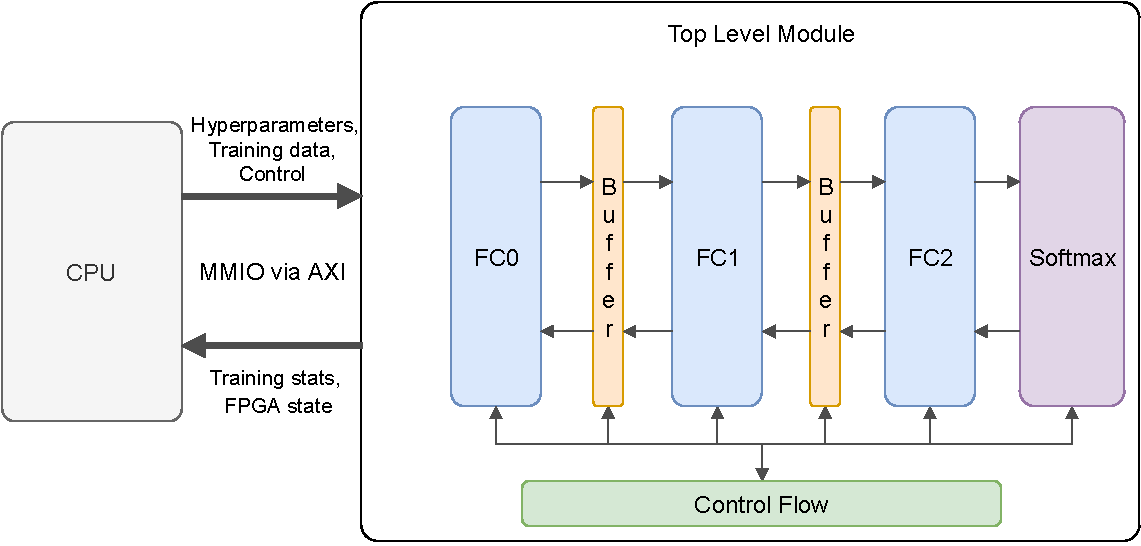
\includegraphics[width=\textwidth]{figures/overall_arch}
	\caption{Architecture of the hardware accelerator}\label{overall-arch}
\end{figure}

\section{Layer Architecture}

\subsection{Fully Connected Layers}

\begin{figure}
	\centering 
	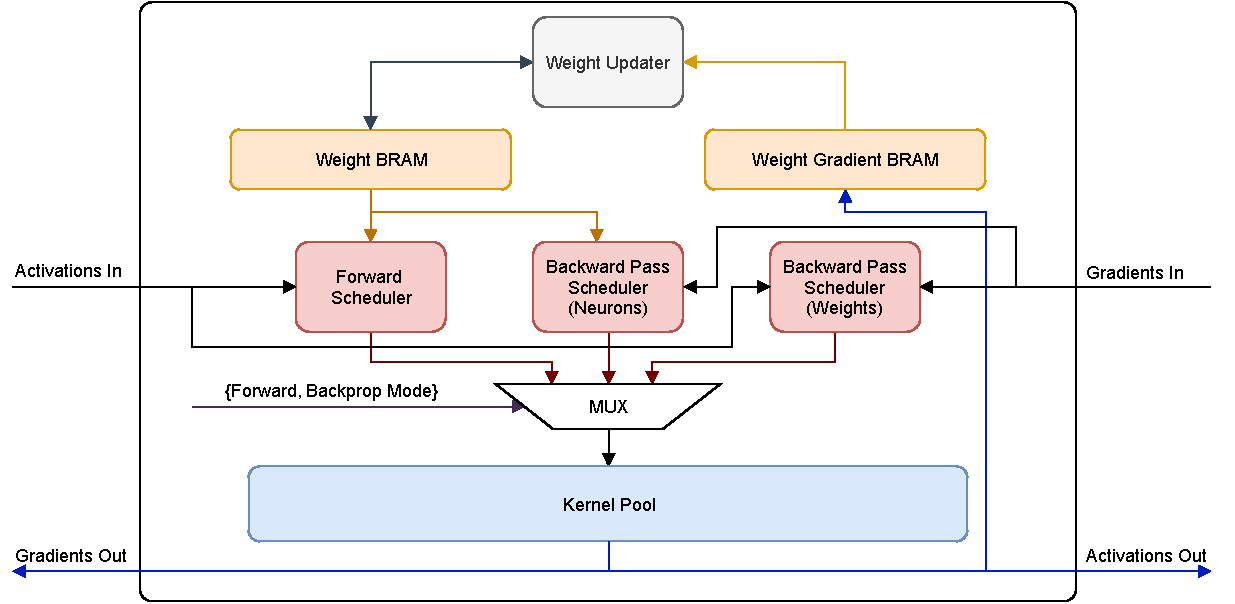
\includegraphics[width=\textwidth]{figures/fully_connected_arch}
	\caption{Architecture of the fully connected layer}\label{fc-arch}
\end{figure}

\begin{figure}
	\centering 
	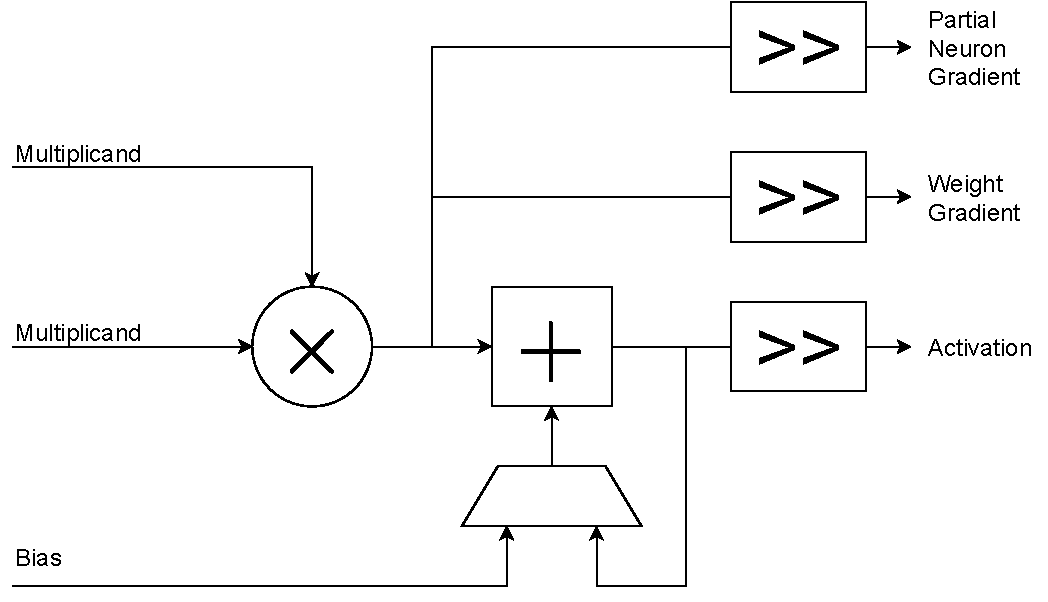
\includegraphics[width=5in]{figures/kernel_arch}
	\caption{Architecture of the kernel}\label{kernel-arch}
\end{figure}

\subsection{Softmax Layer}
To have training be feasible, a proper loss function was required to calculate initial gradients for the output neurons. As such, cross entropy loss, one of the most popular loss functions in deep learning was chosen for this network. Cross-entropy loss is a statistical loss that uses probabilities as input, as shown below.
\begin{align}
\mathcal{L}(y) = - \sum_{i = 1}^{C}y_{i,c}\log(p_{i,c})
\end{align}
In this equation, 
\todo[inline]{Consider against the cross entropy loss defined in chapter 3, define it in chapter 2 IMO}

As explained in chapter \ref{background}, the softmax functions converts logits to probabilities in following manner

\section{Interlayer Architecture}
\section{ARM-Zynq Communication}
\section{Memory Map Layout}

\section{Project Structure}


\begin{figure}
	\begin{tikzpicture}[]
	\node[] at (0,0) (top) {neural\_net\_top.sv};
	\node[] at (3, -1) (mlled) {fc0\_layer.sv};
	\node[] at (3, -2) (debounce) {debounce.v};
	\node[] at (3, -3) (scope) {red\_pitaya\_scope.v};
	\node[] at (3, -4) (buffermodule) {buffer\_module.v};
	\node[] at (3, -5) (irf) {internal\_ref\_gen.xci};
	\node[] at (3, -6) (pfd) {pfd.v};
	\node[] at (6, -7) (pfdblock) {pfd\_block.v};
	\node[] at (6, -8) (pfdfilter) {pfd\_filter.v};
	\node[] at (3, -9) (freqcounter) {freq\_counter.v};
	\node[] at (6, -10) (freqcounterblock) {freq\_counter\_block.v};
	\node[] at (9, -11) (interp) {freq\_interp\_clk.xci};
	\node[] at (3, -12) (pid) {red\_pitaya\_pid.v};
	\node[] at (6, -13) (pidblock) {imra\_pid\_block.v};
	\node[] at (6, -14) (pidfilt) {iir\_filter.v};
	\node[] at (3, -15) (analog) {red\_pitaya\_analog.v};
	\node[] at (6, -16) (dds) {dds/mixer/lpf};
	
	
	\draw [->] (top) |- (mlled.west);
	\draw [->] (top) |- (debounce.west);
	\draw [->] (top) |- (scope.west);
	\draw [->] (top) |- (buffermodule.west);
	\draw [->] (top) |- (irf.west);
	\draw [->] (top) |- (pfd.west);
	\draw [->] (top) |- (freqcounter.west);
	\draw [->] (top) |- (pid.west);
	\draw [->] (top) |- (analog.west);
	\draw [->] (pfd) |- (pfdblock.west);
	\draw [->] (pfd) |- (pfdfilter.west);
	\draw [->] (freqcounter) |- (freqcounterblock.west);							
	\draw [->] (freqcounterblock) |- (interp.west);
	\draw [->] (pid) |- (pidblock.west);
	\draw [->] (pid) |- (pidfilt.west);
	\draw [->] (analog) |- (dds.west);
	
	
	
	\end{tikzpicture}
	\caption{Hierarchy of the FPGA code used for the implementation of the network.}
\end{figure}